\begin{featurebox}
\caption{The Rules of Engagement for Order-Of-Magnitude Estimates}
This work relies heavily on using so-called "back-of-the-envelope" estimates to 
understand the abundances and growth-rate dependences of a variety of molecular
complexes. This moniker arises from the limitation that any estimate should be
able to fit on the back of a postage envelope. As such, we must draw a set of
rules governing our precision and sources of key values. 

\textbf{\itshape The rule of "one, few, and ten".} The philosophy behind
order-of-magnitude estimates is to provide a estimate of the appropriate scale,
not a prediction with infinite accuracy. As such, we define three different
scales of precision in making the estimates. The scale of "one" is reserved for
values that range between 1 and 2. For example, If a particular process has been
experimentally measured to transport 1.87 protons per second, we approximate
this process to require 2 protons per event. The scale of "few" is reserved for
values ranging between 3 and 5. For example, we will often use Avogadro's number
to compute the number of molecules in a cell given a concentration and a volume.
Rather than using Avogadro's number as $6.02214 \times 10^{23}$, we will
approximate it as $5 \times 10^{23}$. Finally, the scale of "ten" is reserved
for values which we know within an order of magnitude. If a particular protein
complex is present at 883 copies per cell, we say that it is present in
approximately $10^3$ copies per cell. These different scales will be used in
combination to arrive at simple estimates that report the expected scale of the
observed data. Therefore, the estimates  presented here should not be viewed as
hard-and-fast predictions of precise copy numbers, but as approximate lower (or upper)
bounds for the number of complexes that may be needed to satisfy some cellular requirement.

Furthermore, we use equality symbols ($=$) sparingly and frequently defer to
approximation ($\approx$) or scaling ($\sim$) symbols when reporting an
estimate. When $\approx$ is used aside a value, we are implicitly stating that
we are confident in this estimate within a factor of a few. When a scaling
symbol $\sim$ is used, we are stating that we are confident in our estimate to
within an order of magnitude. 

\textbf{\itshape The BioNumbers Database as a source for values.} In making our
point estimates, we often require approximate values for key cellular
properties, such as the elemental composition of the cell, the average dry mass,
or approximate rates of synthesis an polymerization. We rely heavily on the
BioNumbers Database \citep{milo2010} as a repository for such information. Every
value we draw from the BioNumbers Database as an associated BioNumbers ID
number, abbreviated as BNID. When we have used a value from the data base in
making our estimate, we provide this ID number (or numbers, depending on the
quantity) in parentheses on in grey-boxes in the figures. For some processes,
values needed to complete the estimate were not present in the data base. In
these cases, we turned to the original literature and have provided citations to
the appropriate references from where the value was obtained. 

\textbf{\itshape Uncertainty in the data sets and the accuracy of an estimate.}
The data sets presented analyzed in this work are the products of extremely
careful experimentation with the aim to report, to the best of their ability,
the absolute copy numbers of proteins in the cell. These data, collected over
the span of a few years, come from different labs and use different internal
standards, controls, and even techniques. As a result, there is notable
disagreement in the observed copy numbers for some complexes between the
different data sets. In assessing whether our estimates could explain the
observed scales and growth-rate dependencies, we considered the degree of
variation between the different data sets. For example, say a particular
estimate undercuts the observed data by an order of magnitude. If all data sets
agree within a factor of a few of each other, we revisit our estimate and
consider what me may have missed. However, if the data sets themselves disagree
by an order of magnitude between them, we determine that our estimate is
appropriate given the variation in the data.
\label{box:estimate_rules}
\end{featurebox}


\section{Uptake of Nutrients}
We begin our series of estimates by considering the critical transport
processes diagrammed in \FIG{categories}(A). In order to build new cellular
mass, the molecular and elemental building blocks must be scavenged from the
environment in different forms. Carbon, for example, is acquired via the
transport of carbohydrates and sugar alcohols with some carbon sources
receiving preferential treatment in their consumption \citep{monod1947}.
Phosphorus, sulfur, and nitrogen, on the other hand, are harvested primarily
in the forms of inorganic salts, namely phosphate, sulfate, and ammonia
\citep{jun2018, assentoft2016, stasi2019, antonenko1997, rosenberg1977,
willsky1973}. All of these compounds have different permeabilities across the
cell membrane \cite{phillips2018} and most require some energetic investment
either via ATP hydrolysis or through the proton electrochemical gradient to
bring the material across the hydrophobic cell membrane. Given the diversity
of biological transport mechanisms and the vast number of inputs needed to
build a cell, we begin by considering transport of some of the most important
cellular ingredients: carbon, nitrogen, oxygen, hydrogen, phosphorus, and
sulfur.

The elemental composition of \textit{E. coli} has received much quantitative
attention over the past half century \citep{neidhardt1991, taymaz-nikerel2010,
heldal1985, bauer1976}, providing us with a starting point for estimating the
copy numbers of various transporters. While there is some variability in the
exact elemental percentages (with different uncertainties), we can estimate that
the dry mass of a typical \textit{E. coli} cell is $\approx$ 45\% carbon
(BioNumber ID: 100649, see \BOX{estimate_rules}), $\approx$ 15\% nitrogen (BNID: 106666), $\approx$ 3\% phosphorus (BNID: 100653), and
1\% sulfur (BNID: 100655).In the coming paragraphs, we will
engage in a dialogue between back-of-the-envelope estimates for the numbers of
transporters needed to facilitate these chemical stoichiometries and the
experimental proteomic measurements of the biological reality. Such an approach
provides the opportunity to test if our biological knowledge is sufficient to
understand the scale at which these complexes are produced. At the end of this
section, we discuss physical limits as to the number of transporters that can be
present, and comment on the plausibility of this process acting as a molecular bottleneck.

\subsection{Nitrogen Transport}
We must first address which elemental sources must require proteinaceous
transport, meaning that the cell cannot acquire appreciable amounts simply
via diffusion across the membrane. The permeability of the lipid membrane to
a large number of solutes has been extensively characterized over the past
century. Large, polar molecular species (such as various sugar molecules,
sulfate, and phosphate) have low permeabilities while small, non-polar
compounds (such as oxygen, carbon dioxide, and ammonia) can readily diffuse
across the membrane. Ammonia, a primary source of nitrogen in typical
laboratory conditions, has a permeability on par with water ($\sim 10^5$
nm/s, BNID:110824). In particularly nitrogen-poor conditions,
\textit{E. coli} expresses a transporter (AmtB) which appears to aid in
nitrogen assimilation, though the mechanism and kinetic details of transport
are still a matter of debate \citep{heeswijk2013a, khademi2004}. Beyond
ammonia, another plentiful source of nitrogen come in the form of glutamate,
which has its own complex metabolism and scavenging pathways. However,
nitrogen is plentiful in the growth conditions examined in this work,
permitting us to neglect nitrogen transport as a potential rate limiting
process in cell division in typical experimental conditions. We direct the
reader to the Supplemental Information for a more in-depth discussion of
permeabilities and a series of calculations revealing that active nitrogen
transport can be neglected for the purposes of this article.

\subsection{Carbon Transport}
We begin with the most abundant element in \textit{E. coli}
by mass, carbon. Using $\approx$ 0.3 pg as the typical \textit{E. coli} dry
mass (BNID: 103904), we estimate that $\sim 10^{10}$
carbon atoms must be brought into the cell in order to double all of the
carbon-containing molecules (\FIG{carbon_tport}(A, top)). Typical laboratory
growth conditions, such as those explored in the aforementioned proteomic
data sets, provide carbon as a single class of sugar such as glucose,
galactose, or xylose to name a few. \textit{E. coli} has evolved myriad
mechanisms by which these sugars can be transported across the cell membrane.
One such mechanism of transport is via the PTS system which is a highly
modular system capable of transporting a diverse range of sugars
\citep{escalante2012}. The glucose-specific component of this system
transports $\approx$ 200 glucose molecules per second per transporter (BNID:
114686). Making the assumption that this is a typical sugar
transport rate, coupled with the need to transport $\sim 10^{10}$ carbon atoms, we
arrive at the conclusion that on the order of 1,000 transporters must be
expressed in order to bring in enough carbon atoms to divide in 5000 s,
diagrammed in the top panel of \FIG{carbon_tport}(A). This estimate, along
with the observed average number of the PTS system carbohydrate transporters present in the
proteomic data sets \citep{schmidt2016, peebo2015,valgepea2013,li2014}, is
shown in \FIG{carbon_tport}(A). While we estimate 1500 transporters are
needed with a 5000 s division time, we can abstract this calculation to consider
any particular growth rate given knowledge of the cell density and volume as a
function of growth rate and direct the reader to the Supplemental Information for more information. As
revealed in \FIG{carbon_tport}(A), experimental measurements exceed the estimate
by several fold, illustrating that transport of carbon into the cell is not
rate limiting for cell division. Abstracting this point estimate at 5000 s to a
continuum of growth rates (grey line in \FIG{carbon_tport}(A)) reveals an excess
of transporters at other growth rates, though in rapid growth regimes, the
abundance is below our simple estimate.
\begin{figure}
    \begin{fullwidth}
    \centering{
    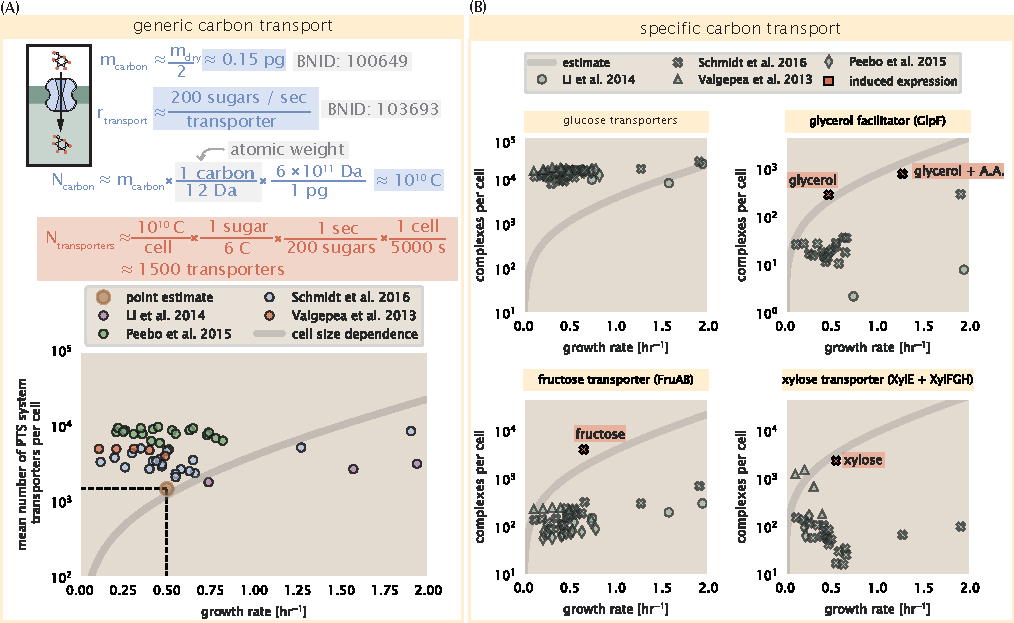
\includegraphics{main_figs/fig2_carbon_transport.pdf}
    \caption{\textbf{The abundance of carbon transport systems across growth
    rates.} (A) A simple estimate for the minimum number of generic carbohydrate
    transport systems (top) assumes $\sim 10^{10}$ C are needed to complete
    division, each transported sugar contains $\approx 5$ C, and each
    transporter conducts sugar molecules at a rate of $\approx 200$ per second.
    Bottom plot shows the estimated number of transporters needed at a growth
    rate of $\approx 0.5 $ per hr (light-brown point and dashed lines).  Colored
    points correspond to the mean number of complexes involved in carbohydrate import
    (complexes annotated with the Gene Ontology terms GO:0009401 and GO:0098704) for
    different growth conditions across different published datasets. (B) The
    abundance of various specific carbon transport systems plotted as a function
    of the population growth rate. The rates of substrate transport to compute
    the continuum growth rate estimate (grey line) were 200 glucose$\cdot$
    s$^{-1}$ (BNID: 103693),  2000 glycerol$\cdot$s$^{-1}$
    \citep{lu2003}, 200 fructose$\cdot$
    s$^{-1}$ (assumed to be similar to PtsI, BNID: 103693), and 50 xylose$\cdot$s$^{-1}$
    (assumed to be comparable to LacY, BNID:103159).
    Red points and highlighted text indicate conditions in
    which the
    only source of carbon in the growth medium induces expression of the
    transport system. Grey line in (A) and (B) represents the estimated number of transporters per cell at a continuum
    of growth rates.}
    \label{fig:carbon_tport}
    }
    \end{fullwidth}
\end{figure}

The estimate presented in \FIG{carbon_tport}(A) neglects any specifics of the
regulation of the carbon transport system and presents a  view of how
many carbohydrate transporters are present on average. Using the diverse array
of growth conditions explored in the proteomic data sets, we can explore how
individual carbon transport systems depend on the population growth rate. In
\FIG{carbon_tport}(B), we show the total number of carbohydrate transporters
specific to different carbon sources. A striking observation, shown in the
top-left plot of \FIG{carbon_tport}(B), is the constancy in the expression of the
glucose-specific transport systems. Additionally, we note that the total number
of glucose-specific transporters is tightly distributed at $\approx 10^4$ per cell,
the approximate number of transporters needed to sustain rapid growth of several
divisions per hour. This
illustrates that \textit{E. coli} maintains a substantial number of complexes
present for transporting glucose regardless of growth rate, which is known to be the preferential carbon
source \citep{monod1947, liu2005a, aidelberg2014}.

It is now understood that a large number of metabolic operons are regulated
with dual-input logic gates that are only expressed when glucose
concentrations are low (mediated by cyclic-AMP receptor protein CRP) and the
concentration of other carbon sources are elevated \citep{gama-castro2016,
zhang2014a}. A famed example of such dual-input regulatory logic is in the
regulation of the \textit{lac} operon which is only natively activated in the
absence of glucose and the presence of allolactose, an intermediate in
lactose metabolism \citep{jacob1961}, though we now know of many other such
examples \citep{ireland2020, gama-castro2016, belliveau2018}. This
illustrates that once glucose is depleted from the environment, cells have a
means to dramatically increase the abundance of the specific transporter
needed to digest the next sugar that is present. Several examples of induced
expression of specific carbon-source transporters are shown in
\FIG{carbon_tport}(B). Points colored in red (labeled by red text-boxes)
correspond to growth conditions in which the specific carbon source
(glycerol, xylose, or fructose) is present. These plots show that, in the
absence of the particular carbon source, expression of the transporters is
maintained on the order of $\sim 10^2$ per cell. However, when the transport
substrate is present, expression is induced and the transporters become
highly-expressed. The grey lines in \FIG{carbon_tport}(B) show the estimated
number of transporters needed at each growth rate to satisfy the cellular
carbon requirement. It is notable that in all cases, the magnitude of induced
expression (shown in red) falls close to the estimate, illustrating the
ability of the cell to tune expression in response to changing environments.
Together, this generic estimation and the specific examples of induced
expression suggest that transport of carbon across the cell membrane, while
critical for growth, is not the rate-limiting step of cell division.

\subsection{Phosphorus and Sulfur Transport}
We now turn our attention towards other essential elements, namely phosphorus and
sulfur. Phosphorus is critical to the cellular energy economy in the form of
high-energy phosphodiester bonds making up DNA, RNA, and the NTP energy pool as
well as playing a critical role in the post-translational modification of
proteins and defining the polar-heads of lipids. In total, phosphorus
makes up $\approx$3\% of the cellular dry mass which in typical experimental conditions is in the form of inorganic phosphate. The cell membrane
has remarkably low permeability to this highly-charged and critical molecule,
therefore requiring the expression of active transport systems. In \textit{E. coli}, the proton
electrochemical gradient across the inner membrane is leveraged to transport
inorganic phosphate into the cell \citep{rosenberg1977}.
Proton-solute symporters are widespread in \textit{E. coli} \citep{ramos1977,
booth1979} and can have rapid transport rates of 50 to 100 molecules per second for
sugars and other solutes (BNID: 103159; 111777). As a more
extreme example, the proton transporters in the F$_1$-F$_0$ ATP synthase, which
use the proton electrochemical gradient for rotational motion, can shuttle
protons across the membrane at a rate of $\approx$ 1000 per second (BNID:
104890; 103390). In \textit{E.
coli} the PitA phosphate transport system has been shown to be very tightly coupled
with the proton electrochemical gradient with a 1:1 proton:phosphate
stoichiometric ratio \citep{harris2001, feist2007}. Taking the geometric mean of
the aforementioned estimates gives a plausible rate of phosphate transport on
the order of 300  per second. Illustrated in
\FIG{phospho_sulfo_tport}(A), we can estimate that $\approx$ 200 
phosphate transporters are necessary to maintain an $\approx$ 3\% dry mass with
a 5000 s division time. This estimate is consistent with observation when we examine the
observed copy numbers of PitA in proteomic data sets (plot in
\FIG{phospho_sulfo_tport}(A)). While our estimate is very much in line with the
observed numbers, we emphasize that this is likely a slight overestimate of the
number of transporters needed as there are other phosphorous scavenging systems,
such as the ATP-dependent phosphate transporter Pst system which we have neglected.

Satisfied that there are a sufficient number of phosphate transporters
present in the cell, we now turn to sulfur transport as another potentially rate
limiting process. Similar to phosphate, sulfate is  highly-charged
and not particularly membrane permeable, requiring active
transport. While there exists a H+/sulfate symporter in \textit{E.
coli}, it is in relatively low abundance and is not well characterized
\citep{zhang2014}. Sulfate is predominantly acquired via the ATP-dependent ABC
transporter CysUWA system which also plays an important role in selenium
transport \citep{sekowska2000, sirko1995}. While specific kinetic details of
this transport system are not readily available, generic ATP transport
systems in prokaryotes transport on the order of 1 to 10 molecules per second
(BNID: 109035). Combining this generic
transport rate, measurement of sulfur comprising 1\% of dry mass, and a 5000
second division time yields an estimate of $\approx$ 1000 CysUWA
complexes per cell (\FIG{phospho_sulfo_tport}(B)). Once again, this estimate
is in notable agreement with proteomic data sets, suggesting that there are
sufficient transporters present to acquire the necessary sulfur. In a similar
spirit of our estimate of phosphorus transport, we emphasize that this is
likely an overestimate of the number of necessary transporters as we have
neglected other sulfur scavenging systems that are in lower abundance.


\begin{figure*}
    \begin{fullwidth}
    \centering{
        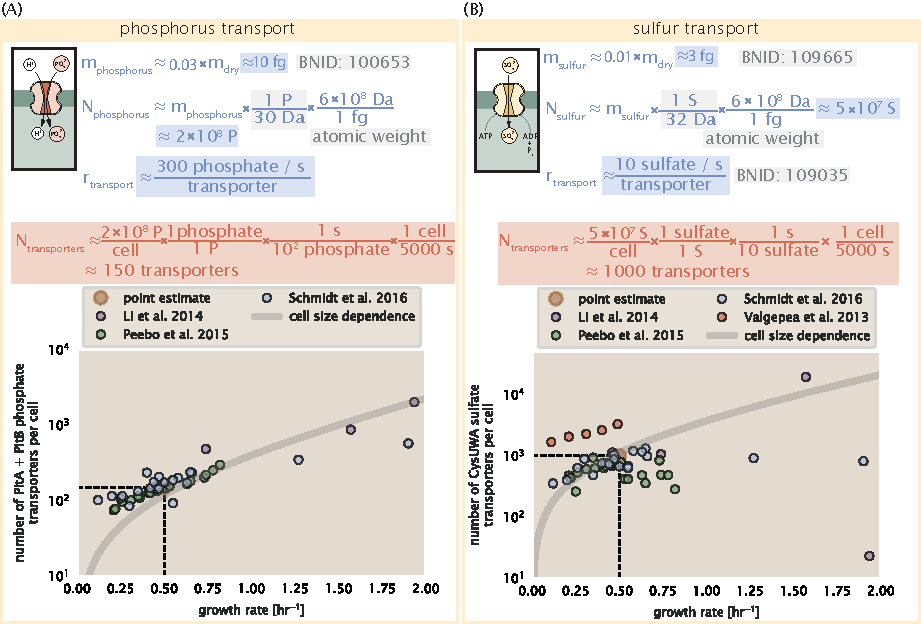
\includegraphics{main_figs/fig3_phospho_sulfo_transport.pdf}
        \caption{\textbf{Estimates and measurements of phosphate and sulfate
        transport systems as a function of growth rate.} (A) Estimate for the
        number of PitA phosphate transport systems needed to maintain a 3\%
        phosphorus \textit{E. coli} dry mass. Points in plot correspond to
        the the total number of PitA transporters per cell. (B) Estimate of
        the number of CysUWA complexes necessary to maintain a 1\% sulfur
        \textit{E. coli} dry mass. Points in plot correspond to average
        number of CysUWA transporter complexes that can be formed given the
        transporter stoichiometry [CysA]$_2$[CysU][CysW][Sbp/CysP]. Grey line
        in (A) and (B) represents the estimated number of transporters per
        cell at a continuum of growth rates.}
        \label{fig:phospho_sulfo_tport}
    }
    \end{fullwidth}
\end{figure*}


\subsection{Limits on Transporter Expression}
So which, if any, of these processes may be rate limiting for growth? As
suggested by \FIG{carbon_tport} (B), induced expression can lead to an
order-of-magnitude (or more) increase in the amount of transporters needed to
facilitate transport. Thus, if acquisition of nutrients was the limiting state
in cell division, could expression simply be increased to accommodate faster
growth? A way to approach this question is to compute the amount of space in the
bacterial membrane that could be occupied by nutrient transporters. Considering a rule-of-thumb for the surface area of
\textit{E. coli} of about 5 \textmu m$^2$ (BNID: 101792), we expect
an areal density for 1000 transporters to be approximately 200
transporters/ \textmu m$^2$. For a typical transporter occupying about 50
nm$^2$/dimer, this amounts to about only 1 percent of the total inner membrane
\citep{szenk2017}. In addition, bacterial cell membranes typically have
densities of 10$^5$ proteins/$\mu m^2$ \citep{phillips2018}, implying that the
cell could accommodate more transporters of a variety of species if it were rate
limiting. As we will see in the next section, however, occupancy of the membrane can
impose other limits on the rate of energy production.
